% 2021 全国乙卷理科第 9 题：海岛测高示意图；逻辑图名 2021-national-b-science-t09-island
% 依据 PDF 第 1 页；A、E、H、G、C 共线，DE=FG，B-D-H 与 B-F-C 共线。
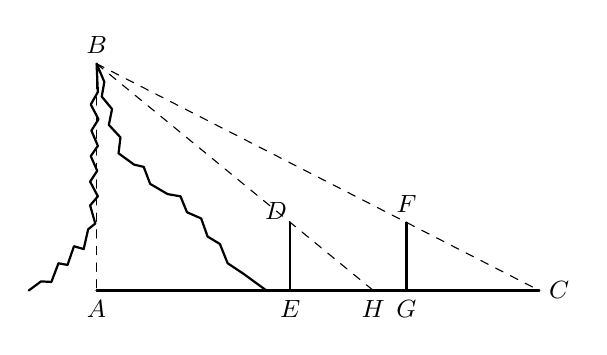
\begin{tikzpicture}[x=0.82cm,y=0.72cm,line cap=round,line join=round,font=\small]
  \coordinate (A) at (0,0);
  \coordinate (B) at (0,4);
  \coordinate (E) at (3,0);
  \coordinate (D) at (3,1.2);
  \coordinate (H) at (4.286,0);
  \coordinate (G) at (4.8,0);
  \coordinate (F) at (4.8,1.2);
  \coordinate (C) at (6.857,0);

  % Island outline and measured height
  \draw[thick]
    (-1.05,0) -- (-0.86,0.16) -- (-0.70,0.15) -- (-0.59,0.48)
    -- (-0.45,0.45) -- (-0.35,0.78) -- (-0.20,0.73) -- (-0.13,1.08)
    -- (-0.02,1.18) -- (-0.10,1.50) -- (0.02,1.66) -- (-0.10,1.92)
    -- (0.01,2.11) -- (-0.09,2.37) -- (0.02,2.55) -- (-0.08,2.82)
    -- (0.03,3.02) -- (-0.09,3.28) -- (0.02,3.50) -- (0,4)
    -- (0.12,3.68) -- (0.08,3.42) -- (0.24,3.20) -- (0.19,2.92)
    -- (0.37,2.70) -- (0.34,2.42) -- (0.58,2.22) -- (0.73,2.18)
    -- (0.83,1.88) -- (1.10,1.70) -- (1.30,1.66) -- (1.40,1.38)
    -- (1.62,1.27) -- (1.72,0.95) -- (1.91,0.82) -- (2.03,0.48)
    -- (2.28,0.29) -- (2.63,0);
  \draw[dashed] (B) -- (A);

  % Horizontal reference line, equal poles and sight lines
  \draw[thick] (A) -- (C);
  \draw[dashed] (B) -- (H);
  \draw[dashed] (B) -- (C);
  \draw[thick] (D) -- (E);
  \draw[thick] (F) -- (G);

  \node[above] at (B) {$B$};
  \node[below] at (A) {$A$};
  \node[above left,inner sep=1pt] at (D) {$D$};
  \node[below] at (E) {$E$};
  \node[below] at (H) {$H$};
  \node[above] at (F) {$F$};
  \node[below] at (G) {$G$};
  \node[right] at (C) {$C$};
\end{tikzpicture}
